\documentclass{TIJMUjiaoanLL}
\pagestyle{empty}


\begin{document}


%课程名称
\kecheng{系统生物学}
%课程内容
\neirong{基因组学(测序技术简介)\ /\ 第2章}
%教师姓名
\jiaoshi{伊现富}
%职称
\zhicheng{讲师}
%教学日期(格式:XXXX年XX月XX日XX时-XX时)
\riqi{2016年9月12日13:30-15:30}
%授课对象(格式:XXX系XXXX年级XX班(硕/本/专科))
\duixiang{生物医学工程与技术学院2013级生信班(本)}
%听课人数
\renshu{28}
%授课方式
\fangshi{理论讲授}
%学时数
\xueshi{2}
%教材版本
\jiaocai{系统生物学,第1版}


%教案首页
\firstHeader
\maketitle
\thispagestyle{empty}

\mudi{
\begin{itemize}
  \item 掌握Sanger测序、Illumina/Solexa测序的主要原理和基本步骤,外显子组测序的实验流程和分析过程。
  \item 熟悉化学测序法、Roche/454测序、ABI/SOLiD测序的主要原理和基本步骤。
  \item 了解tSMS、SMRT、FRET、Nanopore等第三代测序技术。
  \item 自学第三代测序技术的主要原理和基本步骤。
\end{itemize}
}

\fenpei{
\begin{itemize}
  \item (5')引言与导入:介绍测序的基本概念,总结三代测序技术的发展历程。
  \item (10')第一代测序技术:介绍第一代测序技术,讲解化学测序法和Sanger测序法的主要原理。
  \item (40')第二代测序技术:介绍第二代测序技术,讲解Roche/454、Illumina/Solexa、ABI/SOLiD三种测序技术的主要原理和基本步骤,介绍Ion Torrent测序技术,对第二代测序技术进行比较与总结。
  \item (20')第三代测序技术:介绍第三代测序技术,讲解tSMS、SMRT、FRET、Nanopore、TEM等技术的主要原理,对第三代测序技术进行比较与总结。
  \item (10')测序技术比较:对三代测序技术进行总结,从通量、读长、准确性、优缺点等方面对常见的测序技术进行比较。
  \item (10')外显子组测序:简单介绍exome、WES、WGS等概念,讲解外显子组测序的实验步骤和生物信息学分析流程。
  \item (5')总结与答疑:总结授课内容中的知识点与技能,解答学生疑问。
\end{itemize}
}

\zhongdian{
\begin{itemize}
  \item 重点:Illumina/Solexa测序技术的原理和步骤,各种测序技术的优缺点,外显子组测序的分析流程。
  \item 难点:Illmunia/Solexa测序技术的原理和步骤。
  \item 解决策略:通过实例讲解和比较类比帮助学生理解、记忆,播放动画视频帮助学生直观理解复杂原理。
\end{itemize}
}

\waiyu{
  \vspace*{-10pt}
  \begin{multicols}{2}
    DNA测序(DNA sequencing)

    焦磷酸测序(pyrosequencing)

    乳液PCR(emulsion PCR,emPCR)

    桥式扩增(bridge amplification)

    边合成边测序(sequencing by synthesis,SBS)

    边连接边测序(sequencing by ligation)

    外显子组测序(whole exome sequencing,WES)

    基因组测序(while genome sequencing,WGS)
  \end{multicols}
  \vspace*{-10pt}
}

\fuzhu{
\begin{itemize}
  \item 多媒体:主要测序技术的原理和过程,测序技术的发展和比较。
  \item 板书:外显子组测序的分析流程。
\end{itemize}
}

\sikao{
  \vspace*{-10pt}
  \begin{multicols}{2}
  \begin{itemize}
    \item 阐述Sanger测序的主要原理。
    \item 列举第二代测序技术的常见技术。
    \item 阐述Illumina/Solexa测序技术的主要原理。
    \item 列举第三代测序技术的常见技术。
    \item 比较三代测序技术中常见的常见技术。
    \item 总结外显子组测序的分析流程。
  \end{itemize}
  \end{multicols}
  \vspace*{-10pt}
}

\cankao{
\begin{itemize}
  \item 维基百科等网络资源。
\end{itemize}
}

\firstTail


%教案续页
\newpage
\otherHeader

\parpic[fr]{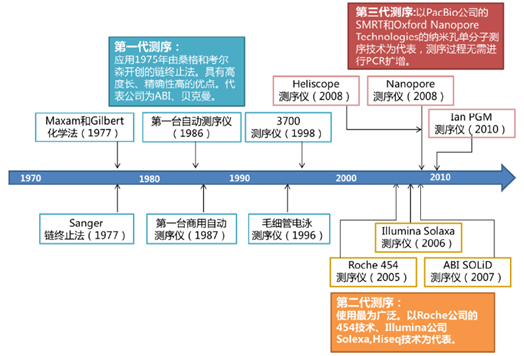
\includegraphics[width=8cm]{c2.sequencing.timeline.02.png}}
\begin{enumerate}
  \item 引言与导入(5分钟)
    \begin{enumerate}
      \item 基本概念
        \begin{itemize}
          \item DNA测序:分析ACGT的排列方式
          \item RNA测学:RNA $\Rightarrow$ cDNA $\Rightarrow$ DNA测序
        \end{itemize}
      \item 测序历史
        \begin{itemize}
          \item 历史发展:第一代 $\Rightarrow$ 第二代 $\Rightarrow$ 第三代
          \item 第一代测序:毛细管电泳测序
          \item 第二代测序:高通量测序
          \item 第三代测序:单分子测序
        \end{itemize}
    \end{enumerate}

  \item 第一代测序技术(10分钟)
\parpic[fr]{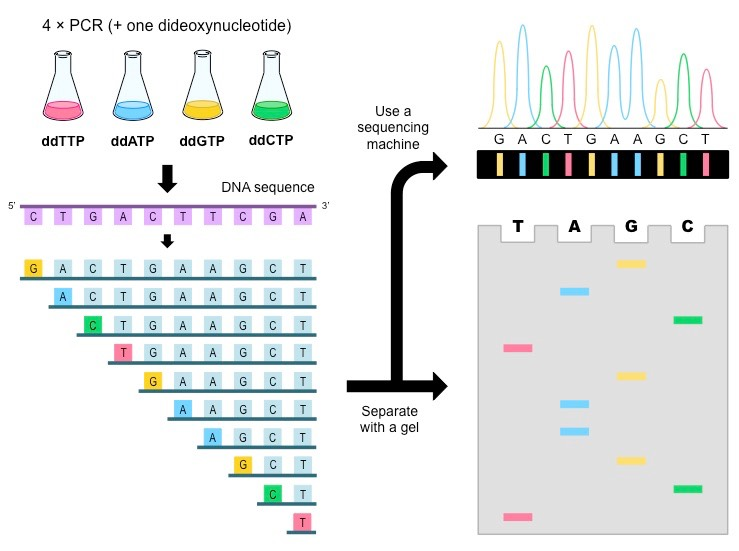
\includegraphics[width=8cm]{c2.sequencing.sanger.05.jpg}}
    \begin{enumerate}
      \item 化学测序法:化学变性
        \begin{itemize}
          \item 1977,Gilbert \& Maxam
          \item 化学测序法(Maxam-Gilbert法)
        \end{itemize}
      \item Sanger测序法:ddNTP,“黄金标准”
        \begin{itemize}
          \item 1975,Sanger \& Coulson
          \item Sanger测序法(双脱氧链终止法)
        \end{itemize}
    \end{enumerate}

  \item 第二代测序技术(40分钟)
    \begin{enumerate}
      \item Roche/454
        \begin{itemize}
          \item 扩增:乳液PCR
          \item 测序:焦磷酸测序
        \end{itemize}
      \item \textcolor{red}{【重点、难点】}Illumina/Solexa \textcolor{red}{(动画演示,详细讲解)}
\parpic[fr]{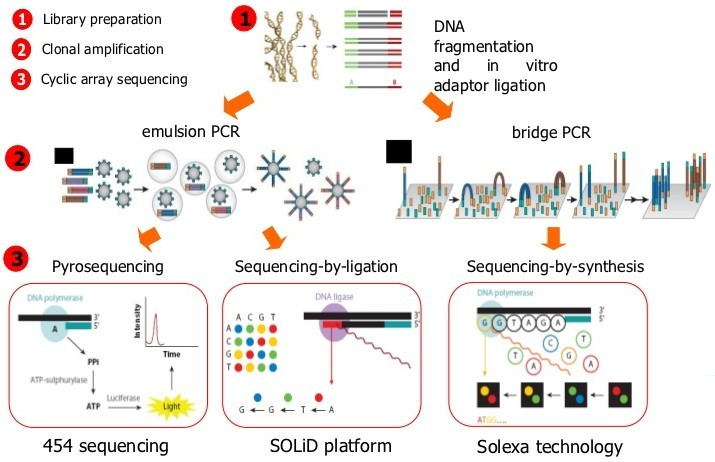
\includegraphics[width=11cm]{c2.sequencing.ngs.01.jpg}}
        \begin{itemize}
          \item 扩增:桥式扩增
          \item 测序:边合成边测序
        \end{itemize}
      \item ABI/SOLiD
        \begin{itemize}
          \item 扩增:乳液PCR
          \item 测序:边连接边测序
        \end{itemize}
      \item 离子半导体测序
      \item \textcolor{red}{【重点】}第二代测序技术比较
    \end{enumerate}
\parpic[fl]{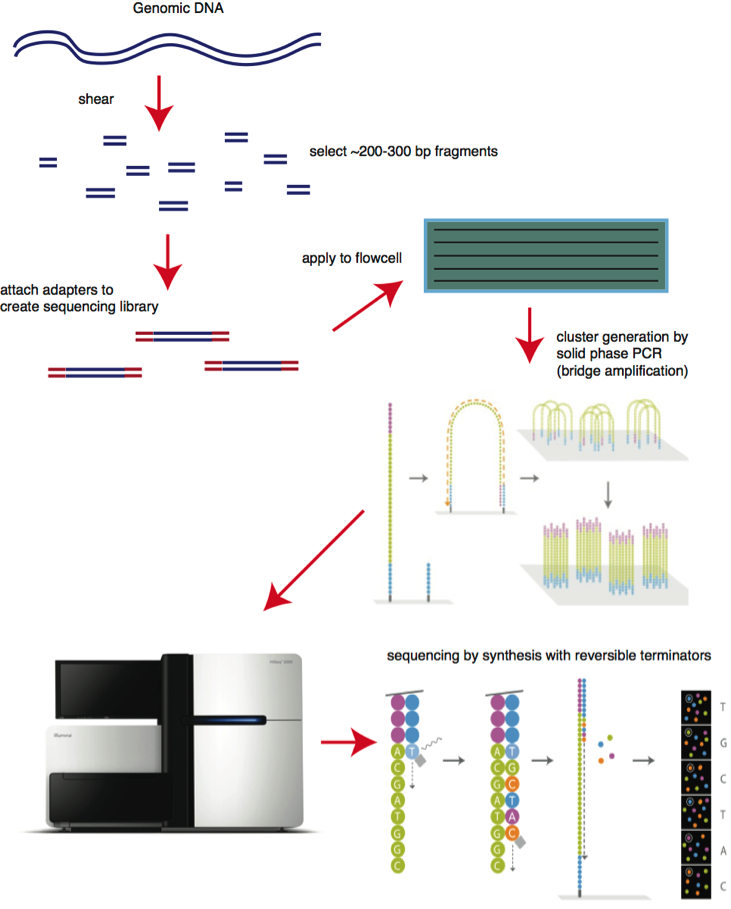
\includegraphics[width=5.8cm,height=8.05cm]{c2.sequencing.ill.01.png}}
\vspace{8em}
\parpic[fr]{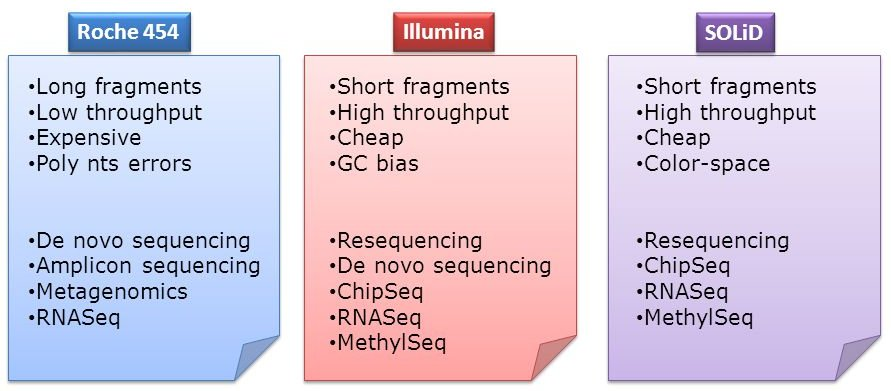
\includegraphics[width=11cm]{c2.sequencing.compare.00.jpg}}
\vspace{0.1em}

\otherTail
\newpage
\otherHeader

\vspace{0.1em}
  \item 第三代测序技术(20分钟)
\parpic[fr]{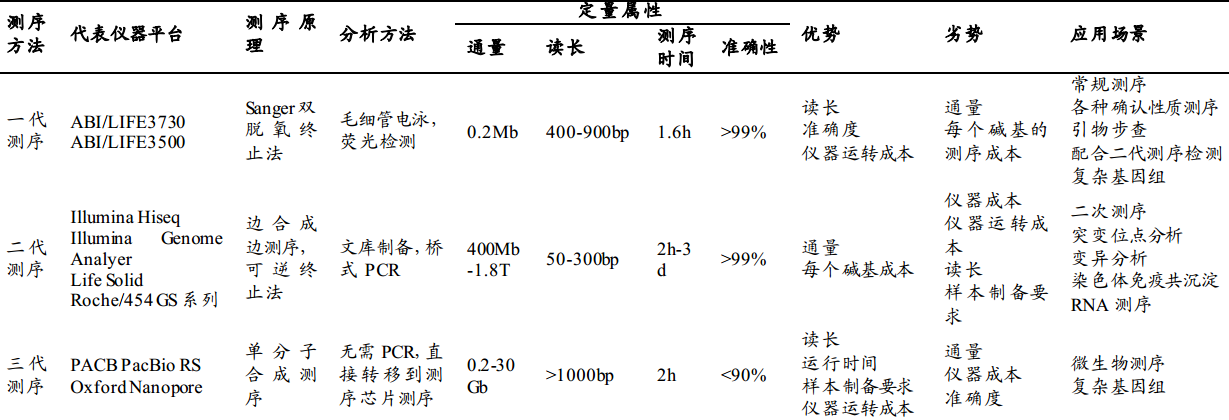
\includegraphics[width=12cm]{c2.sequencing.compare.06.png}}
    \begin{enumerate}
      \item tSMS
      \item SMRT
      \item FRET
      \item Nanopore
      \item TEM
      \item 第三代测序技术比较
    \end{enumerate}
%\parpic[fr]{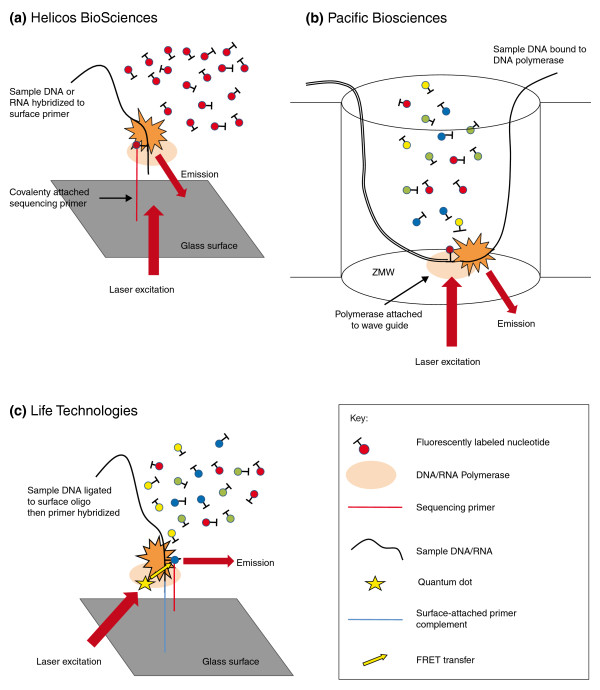
\includegraphics[width=11cm]{c2.sequencing.sms.smrt.fret.01.jpg}}

  \item \textcolor{red}{【重点】}测序技术比较(10分钟)

  \item 外显子组测序(10分钟)
    \begin{enumerate}
\parpic[fr]{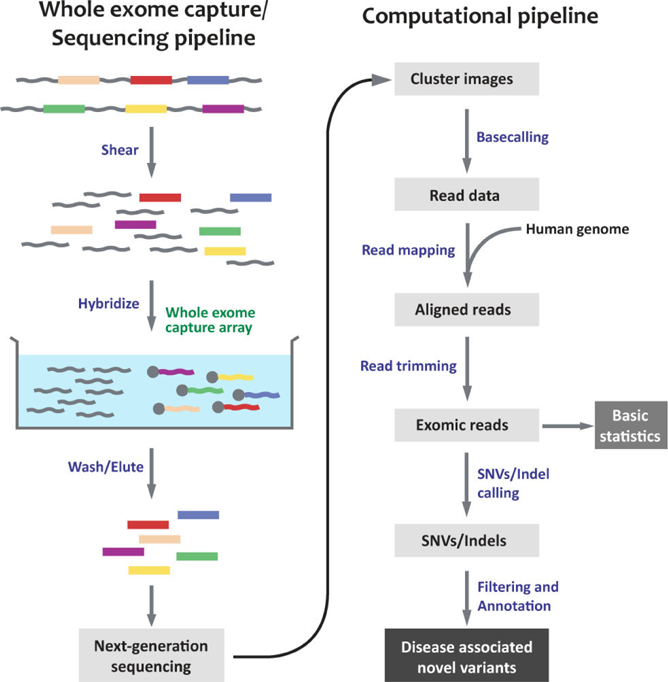
\includegraphics[width=9.5cm]{c2.exome.exp.bx.01.jpg}}
      \item 基本概念
        \begin{itemize}
          \item exome:genome $\Rightarrow$ 1\%,30Mb
          \item WES:exome $\Rightarrow$ sequencing
          \item WGS:genome $\Rightarrow$ sequencing
        \end{itemize}
      \item \textcolor{red}{【重点】}流程:实验 + 分析
    \end{enumerate}

  \item 总结与答疑(5分钟)
    \begin{enumerate}
      \item 知识点
	\begin{itemize}
	  \item 测序技术:第一代,第二代,第三代
	  \item Sanger测序:原理与过程
	  \item Illumina/Solexa测序:原理与过程
	  \item 测序技术比较:优缺点
	  \item 外显子组测序:实验与分析流程
	\end{itemize}
      \item 技能
	\begin{itemize}
	  \item 外显子组测序:数据分析
	\end{itemize}
    \end{enumerate}
\end{enumerate}

\otherTail


\end{document}

